\documentclass[11pt]{article}
\usepackage[margin=1in]{geometry}
\usepackage{booktabs}
\usepackage{graphicx}
\usepackage{amsmath}
\usepackage{siunitx}
\usepackage{xcolor}
\usepackage{caption}
\usepackage[numbers,square]{natbib}
\usepackage[hidelinks]{hyperref}
\captionsetup{font=small,labelfont=bf}
\newcommand{\bc}{bits/char}
\title{\bfseries Morphological embedding factorization helps language models\\
in proportion to a language's morphology}
\author{}
\date{Draft --- internal. Single machine, treebank/subset scale, 2--3 seeds.\\
Read \S\ref{sec:limits} before citing any figure.}

\begin{document}
\maketitle

\begin{abstract}
\noindent
We test whether an explicit morphological prior---factoring a word's input embedding into
a lemma embedding plus an operator for its inflection---improves next-token prediction,
measured in \bc{} of the original text (the only tokenizer-independent measure). In English
the effect is negligible ($-0.011$ \bc). Across five morphologically richer languages it is
20--40$\times$ larger ($-0.19$ to $-0.42$ \bc), scaling with how much of the language is
inflected. A shuffled-root control shows the gain is largely due to the \emph{low-rank
pooling structure} of tying rare word-forms to shared roots, not to the \emph{correctness}
of the morphological grouping---the morphology-specific component is clearly present only in
Turkish. Derivation contributes nothing for a language model in any functional form we
tried, and ``operator as a token'' is strictly worse than ``operator as a pre-model affine
map.'' The paper doubles as a catalogue of measurement traps: nearly every strong effect we
found was, on first measurement, a confound in the direction of our hopes.
\end{abstract}

\section{Introduction}
Language models tokenize with subword schemes---byte-pair encoding and its relatives---that
are optimized for compression, not morphology. A word like Finnish \textit{taloissamme}
(``in our houses'') is shattered into pieces that cut across morpheme boundaries, and every
inflected form of a lemma is estimated largely independently. This is wasteful exactly where
a language inflects heavily: the model must learn each of a lemma's dozens or hundreds of
surface forms as a separate distribution.

We ask a narrow, quantitative question: if we hand the model an explicit morphological prior
---factoring a word's input embedding into a lemma embedding plus a learned operator for its
inflection---does next-token prediction improve, by how much, and \emph{why}? We measure in
\bc{} of the original text, the only measure comparable across tokenizers, and we control the
result three ways: against a byte-fallback BPE baseline that cannot cheat by discarding rare
words; against a pure word-level tokenizer, to separate the tokenizer from the factorization;
and against a shuffled-root null that keeps the factorization's capacity but destroys the
\emph{correctness} of the morphological grouping.

Our contributions are (i) a controlled cross-linguistic measurement showing the prior helps
in proportion to a language's inflection, negligibly in English and 20--40$\times$ more in
five richer languages; (ii) the finding, from the shuffled-root null, that most of the gain
is generic low-rank pooling rather than morphology-specific alignment; (iii) the negative
results that derivation contributes nothing to a language model and that operator-as-token is
worse than operator-as-affine-map; and (iv) a catalogue of measurement traps, since nearly
every effect we report was, on first measurement, a confound in the direction of our
hypothesis.

\section{Related work}
\emph{(Citations reconstructed from memory; venues/pages to be verified against originals.)}

\textbf{Subword tokenization.} BPE \citep{sennrich2016bpe} and
unigram/\textsc{SentencePiece} \citep{kudo2018subword,kudo2018sentencepiece} are the
standard; subword regularization and BPE-dropout \citep{kudo2018subword,provilkov2020bpedropout}
show that tokenization is a modeling choice with real perplexity consequences. Unsupervised
morphological segmentation \citep{creutz2007morfessor} predates the neural era. Our baseline
is byte-level BPE with a byte fallback, and our central metric point is that the apparent
sequence-length cost of word-level tokenization is mostly an \texttt{<unk>}-accounting
artifact (\S\ref{sec:traps}).

\textbf{Morphology-aware and factored embeddings.} Character-aware neural language models
\citep{kim2016charaware} and compositional-morphology embeddings
\citep{botha2014compositional,vania2017characters} build word representations from
sub-lexical structure. Our factorization is deliberately minimal---a lemma embedding plus a
low-rank affine operator per inflection slot, precomputed into an ordinary embedding
table---so it is a structured prior at zero inference cost rather than a runtime character
encoder. The novel component is the \emph{shuffled-root null}, which lets us ask not whether
structure helps but whether the \emph{morphological} structure specifically helps.

\textbf{Multilingual and low-resource morphology.} Massively multilingual models
\citep{devlin2019bert,conneau2020xlmr} and the Universal Dependencies treebanks
\citep{nivre2020ud} make controlled cross-linguistic measurement possible; we use UD's gold
lemma-and-features as the factorization, avoiding an analyzer confound. Our practical
conclusion---that the prior pays most in the data-scarce, morphologically-rich
regime---points at low-resource agglutinative and fusional languages as the setting where it
matters. The companion sense-tokenization experiment (Appendix~\ref{app:sense}) builds on
gloss-based WSD \citep{huang2019glossbert,loureiro2019lmms} over
WordNet/SemCor \citep{fellbaum1998wordnet,miller1993semcor}.

\section{Setup}
\textbf{Metric.} \bc{} over the original characters, counting only characters inside the
scored window. Cross-entropy is \emph{not} comparable across tokenizers (a lexeme stream
contains low-entropy operator tokens), so we never compare it.
\textbf{Baseline.} GPT-2 byte-level BPE, 16k vocab, with a byte fallback so no token is ever
\texttt{<unk>} (\S\ref{sec:traps}). \textbf{Trunk.} A small GPT (L6, $d{=}384$; 10.65M
non-embedding params). Embedding parameters are excluded from ``model size'': they are a
lookup table, zero FLOPs.

\smallskip\noindent\textbf{The factorization.} A word's embedding is
\begin{equation}
e(\text{word}) = E_{\text{root}} + d_{\text{slot}} + U_{\text{slot}}\,(V_{\text{slot}}^{\top} E_{\text{root}}),
\qquad \text{rank } 32,
\end{equation}
with $E_{\text{root}}$ the lemma embedding, $d_{\text{slot}}$ a per-inflection translation,
and $U V^{\top}$ a low-rank rotation. The identity slot is pinned
($d_0{=}0,\,U_0{=}V_0{=}0$) to remove a gauge freedom that otherwise makes the operator
parameters unidentifiable. This precomputes into an ordinary $[V,d]$ table: \textbf{zero
inference FLOPs}. It is a structured prior on the embedding matrix, not a runtime component.

\section{English: the prior barely helps, and derivation not at all}
On wikitext-103, inflection-only factoring (7 operators) beats BPE, and the advantage
\emph{grows as data shrinks} (Table~\ref{tab:ladder}, Fig.~\ref{fig:ladder}). Each arm is
trained to its own best held-out checkpoint under a byte fallback; at the small rung both
arms genuinely converge, so the gain is a fair best-vs-best comparison---though at 10k it is
partly \emph{overfitting resistance}, a legitimate sample-efficiency benefit.

\begin{table}[h]\centering
\caption{English data-efficiency ladder (wikitext-103, byte fallback, best held-out checkpoint, 2 seeds).}
\label{tab:ladder}
\begin{tabular}{lccc}
\toprule
paragraphs & BPE & inflection-factored & $\Delta$ \\
\midrule
10{,}000  & 1.956 & 1.824 & $-0.132$ \\
40{,}000  & 1.771 & 1.689 & $-0.082$ \\
160{,}000 & 1.740 & 1.665 & $-0.075$ \\
\bottomrule
\end{tabular}
\end{table}

\textbf{Derivation contributes nothing.} Adding derivational operators
($\textit{worker}\!\leftarrow\!\textit{work}$, \dots)---as tokens or affine maps, with
rotation allowed, at zero sequence-length cost, composed to depth 4---never beats
inflection-only ($\Delta = -0.001 \pm 0.003$). Seven inflectional operators do all the work;
the 27 derivational operators and the entire 29-relation ``atlas'' buy zero \bc{} for a
language model. (The atlas's \emph{geometric} claims about embedding space survive their
controls; what dies is the inference from ``English has this structure'' to ``an LM benefits
from it.'')

\textbf{Operator as matrix, not token.} A pre-model affine map beats an operator token and
beats a free embedding, and survives its shuffled-root null. A pure translation
($E_{\text{root}}+d_{\text{slot}}$, no rotation) \emph{loses} to a free embedding; the
rotation term is necessary. This contradicts the atlas's ``inflection is a translation''
prediction \emph{inside} a language model: the bias is necessary but not sufficient.

Fig.~\ref{fig:drivers} ranks what drives the English gain: decomposing many \emph{rare}
words costs tokens and buys nothing; the win is decomposing \emph{frequent} forms; false
decompositions matter an order of magnitude less.

\begin{figure}[h]\centering
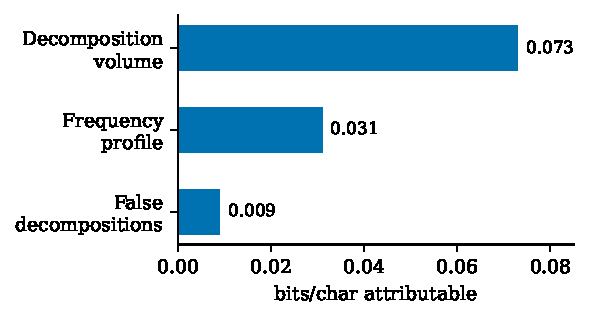
\includegraphics[width=0.62\textwidth]{fig/drivers.pdf}
\caption{Drivers of the English gain. Volume (decomposing rare words) dominates and is a
\emph{cost}, not a benefit; the payoff is in the frequency profile.}
\label{fig:drivers}
\end{figure}

\section{Cross-linguistic: the prior scales with morphology}
Universal Dependencies treebanks (gold lemma\,+\,features $=$ root\,+\,operator; no analyzer
or sandhi confound), 3 seeds. \emph{affine\,--\,free} is the factorization gain;
\emph{affine\,--\,shufroot} (random-root pointing, matched capacity) isolates the
morphology-specific component (Table~\ref{tab:xling}, Fig.~\ref{fig:xling}).

\begin{table}[h]\centering
\caption{Cross-linguistic factorization gain. \emph{affine--free} is the total gain;
\emph{affine--shufroot} is the morphology-specific part (random-root null).}
\label{tab:xling}
\begin{tabular}{lccc}
\toprule
language & \% content-word inflected & affine\,--\,free & affine\,--\,shufroot \\
\midrule
English & 30 & $-0.011$ & $-0.007$ \\
Spanish & 40 & $-0.189$ & $-0.017$ \\
German  & 41 & $-0.216$ & $+0.012$ \\
Turkish & 66 & $-0.359$ & $-0.044$ \\
Russian & 71 & $-0.419$ & $-0.016$ \\
Finnish & 80 & $-0.229$ & $-0.005$ \\
\bottomrule
\end{tabular}
\end{table}

\begin{figure}[h]\centering
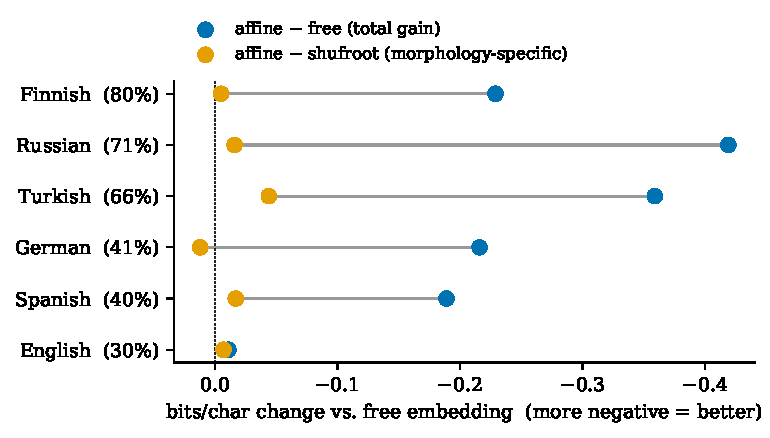
\includegraphics[width=0.82\textwidth]{fig/xling.pdf}
\caption{The total factorization gain (blue) is large in every morphologically rich language
and negligible in English; the morphology-\emph{specific} component (orange, vs.\ a
shuffled-root null) is near zero except in Turkish. Languages ordered by inflection rate.}
\label{fig:xling}
\end{figure}

\begin{figure}[h]\centering
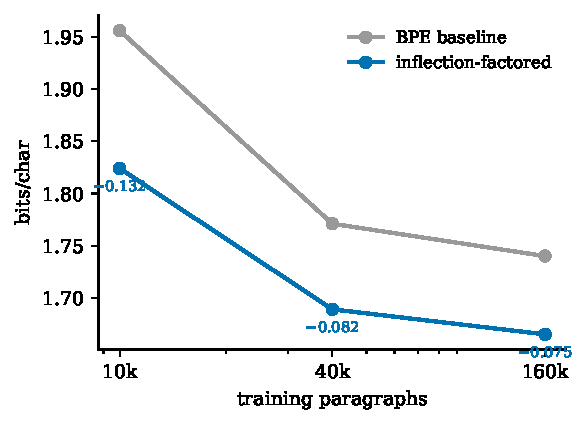
\includegraphics[width=0.60\textwidth]{fig/ladder.pdf}
\caption{English data-efficiency ladder: the advantage over BPE widens as the corpus shrinks.}
\label{fig:ladder}
\end{figure}

\textbf{Finding 1 (robust).} The factorization gain is 20--40$\times$ larger in every rich
language than in English; the ordering is roughly monotonic in inflection rate. English is
close to the \emph{worst} language to demonstrate this on.

\textbf{Finding 1a (the Finnish outlier is corpus size, not morphology).} Finnish is a low
outlier ($-0.229$ at 80\% inflection, below Turkish's $-0.359$ at 66\%) only because its
treebank is 2.3$\times$ larger. The gain is a sample-complexity effect (cf.\ the English
ladder, Fig.~\ref{fig:ladder}): halving the Finnish corpus grows the gain to $-0.391$,
\emph{above} Turkish, restoring monotonicity. The cross-linguistic table therefore conflates
morphological richness with corpus size---a confound (see \S\ref{sec:limits})---but the
resolution reinforces the core claim: less data, bigger gain, in every language.

\textbf{Finding 2 (the honest caveat).} The morphology-specific component is clearly nonzero
only in Turkish; in German it is even slightly positive (shuffled beats real). Most of the
gain is the low-rank pooling structure of tying sparse word-forms to shared roots, which
helps regardless of whether the grouping is the \emph{correct} morphology. We therefore frame
this as \emph{structured sparse embedding factorization helps morphologically rich languages},
not ``morphology is the mechanism.''

\textbf{Finding 3.} Word-level tokenization \emph{alone} loses to BPE in sparse agglutinative
languages (Turkish $+0.155$, Russian $+0.405$, Finnish $+0.218$) because word-forms are too
rare; the factorization is what makes word-level viable there.

\section{Measurement traps (perhaps the real contribution)}
\label{sec:traps}
Nearly every strong effect was, on first measurement, an artifact favoring our hypothesis.
\begin{description}
\item[The \texttt{<unk>} cheat.] BPE mapped out-of-vocab pieces to one frequent
\texttt{<unk>} while \bc{} credited the swallowed word's characters. BPE \texttt{<unk>}'d
5.7\% of tokens, the lexeme stream 2.9\%. Hence the ``20\% length penalty'' was mostly BPE's
cheat (true ratio $1.02\times$), and ``derivation hurts'' was an artifact: the more complete
dictionary escaped less, cheated less, scored worse. A byte fallback fixed both.
\item[Gauge freedom (four times).] A free linear map in front of a structured operator makes
its parameters unidentifiable; a randomly-initialized reflection once scored identically to a
trained one. Pin the identity slot.
\item[No-op nulls.] Shuffling the \emph{targets} of a fitted translation is
permutation-invariant, so the ``null'' scored exactly what the fit scored. Permute the source
or the root assignment.
\item[Confounded arms.] Changing dictionary, escape brackets and operator order in one run,
then crediting whichever had a story. Minimal one-variable contrasts must come first.
\item[Strawman baselines.] Comparing a prototype init (std 0.02) against PyTorch's default
$\mathcal{N}(0,1)$; then leaving \emph{positional} embeddings at $\mathcal{N}(0,1)$ so word
identity was 50$\times$ quieter than position.
\item[Protocol dependence.] The lexeme advantage moves with the LR schedule ($-0.131$ vs.\
$-0.075$ on identical configs). Any \bc{}$\to$params conversion must fix one protocol.
\end{description}

\noindent\textbf{A related negative result.} Initializing the LM's embedding from BERT
contextual prototypes performed \emph{identically to a shuffled permutation} of them; freezing
them cost 0.8 \bc. A good map of a masked LM's representation space is not a good input
parameterization for a causal LM.

\section{Limitations}\label{sec:limits}
Single machine; 2--3 seeds; treebank-scale corpora (17k--518k tokens) for the cross-linguistic
result, a 200k-paragraph wikitext subset for English. \textbf{Corpus size is not controlled
across languages}: the treebanks range 17k--518k tokens, and since the gain is
sample-complexity-driven (Finding 1a), the \emph{affine--free} column conflates morphology
with corpus size---a matched-token cross-linguistic sweep is the needed follow-up. Korean
(no \textsc{feats}), Arabic (lemmatization artifact), and Czech (parse failure) were dropped; the sample is Indo-European-heavy plus Turkish/Finnish. No comparison to
a modern large-vocab BPE at scale or to subword regularization; the trunk is tiny.

\section{Takeaway}
For a causal language model: \textbf{lemmatize and tag inflection.} It is near zero-cost
($1.02\times$ tokens with a byte fallback, zero inference FLOPs), it helps most exactly where
data is scarce and morphology is rich, and it is a structured-pooling effect more than a
linguistic-correctness one. Derivation and the elaborate operator ``language'' we started with
are not worth the complexity for an LM, though they remain valid descriptions of the geometry
of English word embeddings.

\bibliographystyle{plainnat}
\bibliography{refs}

\appendix
\section{A sense-tokenization companion experiment}
\label{app:sense}
A separate exploration asked the dual question for \emph{polysemy}: if morphology makes a
lemma's meaning context-free by pooling its inflected forms, does splitting a word by
\emph{sense} help? We built a coarse sense inventory for 23{,}818 words (2.35 senses/word,
including proper-noun and corpus-specific senses WordNet lacks) with a large model, then
directly tagged 3.26M wikitext occurrences by sense via a batched API run
($\sim$15$\times$ the size of SemCor). The dataset and dictionary are the deliverable; on top
of them we trained two disambiguators and compared them on a common held-out set
(Table~\ref{tab:wsd}).

\begin{table}[h]\centering
\caption{Sense disambiguators on a common 30k held-out set (\emph{balanced} = word whose top
sense is $<$75\% of its occurrences). The trained cross-encoder wins everywhere once the
evaluation is fair; a skew-routed ensemble is worse than the cross-encoder alone.}
\label{tab:wsd}
\begin{tabular}{lccc}
\toprule
disambiguator & all & balanced & skewed \\
\midrule
nearest-centroid propagator (frozen encoder) & 0.743 & --- & --- \\
cross-encoder (target-token readout + target-mask, trained) & \textbf{0.843} & 0.740 & 0.896 \\
skew-routed ensemble & 0.779 & 0.783 & 0.773 \\
\bottomrule
\end{tabular}
\end{table}

Two lessons transfer from the main paper. First, \emph{measure fairly}: the propagator
appeared to win (0.879) under a per-word evaluation that only scored well-populated words; on
a common all-words set it scores 0.743 and the cross-encoder wins cleanly, so the ensemble
built on the propagator's apparent skewed-word strength loses. Second, \emph{point the model
where the signal is}: reading the target word's own contextual token rather than the
sequence \texttt{[CLS]}, and injecting a target-mask embedding (segment-embedding style,
zero-initialized) rather than bracketing the target in text, took balanced-word accuracy from
0.68 to 0.74---the earlier ``0.68 ceiling'' was undertraining and a mis-placed readout, not a
limit. A \emph{cased} backbone did not help: context already carries the disambiguating signal.

\end{document}
